\newpage
\section{Подсистема выгрузки в ТФОМС}

Подсистема выгрузки в ТФОМС позволяет:
\begin{itemize}
 \item 	выгружать из ФТМИС данные о пролеченных пациентах для последующей отправки в ТФОМС;
 \item выгружать из ФТМИС данные об обращениях пациентов для последующей отправки в ТФОМС;
 \item загружать ответы от ТФОМС о принятых или отклоненных случаях обращения;
 \item хранить и просматривать отчеты о выполненных операциях.
\end{itemize}
 
Система позволяет осуществлять выгрузку в форматах:
\begin{itemize}
 \item XML;
 \item DBF.
\end{itemize}
 
Загрузка ответов от ТФОМС осуществляется только в формате XML.
Для корректной выгрузки данных в ТФОМС необходимо настроить шаблоны для выгрузки и другие параметры модуля. Все настройки подсистемы выполняются по нажатию кнопки \btn{Настройки}, расположенной в верхней части любой страницы подсистемы (Рисунок \ref{img_tfoms_main}).

\begin{figure}[ht]\centering
 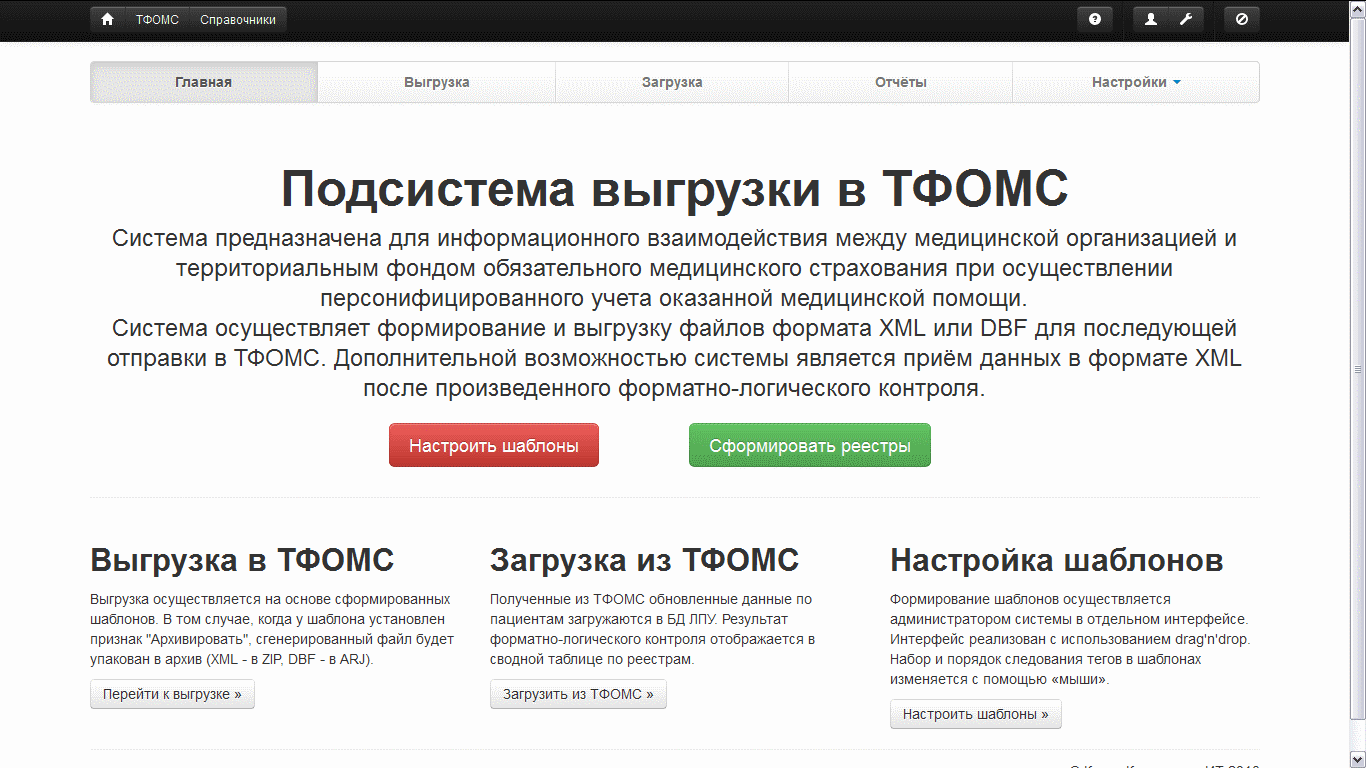
\includegraphics[width = 1\textwidth ,keepaspectratio]{tfoms_main}
 \caption{Главная страница подсистемы выгрузки в ТФОМС}
 \label{img_tfoms_main}
\end{figure}

\subsection{Настройка шаблонов выгрузки}

Для перехода на страницу настройки шаблонов выгрузки необходимо нажать кнопку   в верхней части любой страницы подсистемы и в появившемся меню выбрать пункт \dm{Шаблоны}. Будет осуществлен переход на страницу настройки шаблонов (Рисунок \ref{img_tfoms_unload_conf}). В зависимости от формата выгрузки (XML или DBF) и типа выгружаемых данных необходимо перейти на соответствующую вкладку. Состав управляющих элементов и принцип работы с ними одинаков на каждой из вкладок. Отличие заключается лишь в составе полей для каждого типа выгрузки.

\begin{figure}[ht]\centering
 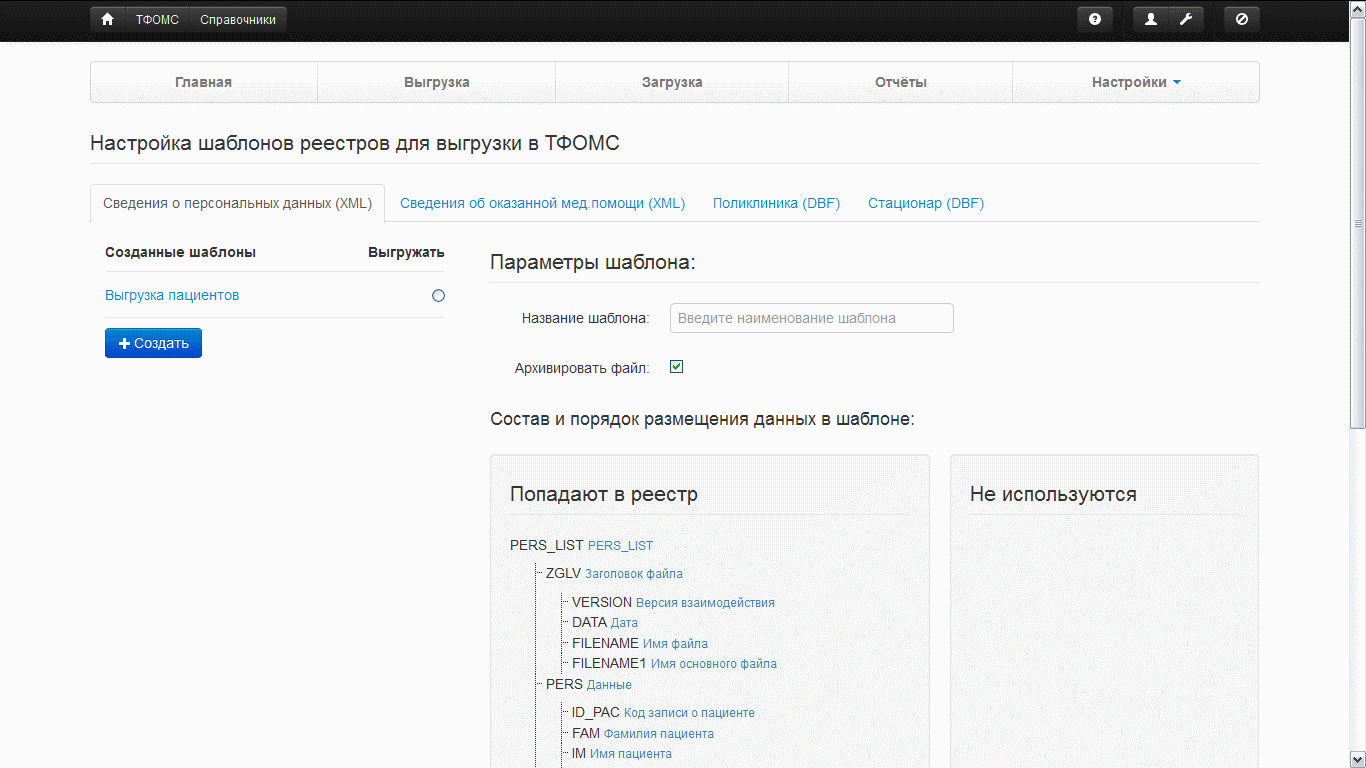
\includegraphics[width = 1\textwidth ,keepaspectratio]{tfoms_unload_conf}
 \caption{Страница настройки шаблонов выгрузки}
 \label{img_tfoms_unload_conf}
\end{figure}

В левом верхнем углу страницы расположен список существующих шаблонов данного типа. В столбце \dm{Выгружать} переключатель должен быть установлен напротив того шаблона, выгрузка по которому будет осуществляться в разделе \dm{Выгрузка}.

Для редактирования шаблона необходимо выделить его название в списке шаблонов в левом верхнем углу, щелкнув по нему левой кнопкой мыши. Параметры шаблона будут отображены и доступны для редактирования в правой части страницы в разделе \dm{Параметры шаблона}. Необходимо отредактировать параметры выгрузки, а затем сохранить шаблон. Для сохранения изменений шаблона следует нажать кнопку \btn{Сохранить} в правом нижнем углу страницы. Если необходимо сохранить измененный шаблон под новым именем, то нужно в поле \dm{Название шаблона} ввести новое имя, а затем нажать кнопку  \btn{Сохранить как новый}. Тогда текущий шаблон останется в прежнем состоянии, а отредактированный шаблон будет сохранен под новым именем, в списке доступных шаблонов появится новая запись.

Для добавления нового шаблона следует нажать кнопку  \btn{Создать}  в левой части страницы, затем следует заполнить параметры шаблона и нажать кнопку \btn{Сохранить} в правом нижнем углу страницы. В списке доступных шаблонов появится новая запись.

Для удаления шаблона нужно выделить его название в списке шаблонов в левом верхнем углу, щелкнув по нему левой кнопкой мыши, а затем нажать кнопку  \btn{Удалить шаблон}. В появившемся диалоговом окне следует подтвердить удаление шаблона. Шаблон будет удален из списка доступных шаблонов в левом верхнем углу.

Для каждого из шаблонов данного раздела задаются следующие параметры:
\begin{itemize}
 \item \dm{Название шаблона} – Имя шаблона, которое будет отображаться в списке доступных шаблонов в левом верхнем углу текущей страницы.
 \item \dm{Архивировать файл} – при установке данного флажка полученный файл будет упакован в zip-архив для файлов XML и в arj-архив для файлов DBF.
 \item \dm{Состав и порядок размещения данных в шаблоне} – в данном разделе необходимо настроить поля, которые должны попадать в выгрузку и порядок их следования. В области \dm{Попадают в реестр} размещаются поля, которые попадают в реестр, в той последовательности, как они должны входить в файл выгрузки. В области \dm{Не используются} размещаются поля, которые не используются в текущей выгрузке. Настройка последовательности полей в шаблоне осуществляется простым перетаскиванием мышью полей в нужную позицию по технологии drag-and-drop.
\end{itemize}

Так как выполнение запроса на сопоставление данных пациентов и оказанных им услуг выполняется достаточно долго, данные последней выборки сначала сохраняются в таблицу AA\_POL, а затем выбираются в файлы выгрузки. После получения ответа от ТФОМС данные о пациентах и услугах так же будут сопоставлены посредством таблицы AA\_POL. Обновление данных в таблице AA\_POL может выполняться как вручную, так и по расписанию (в 2:30 последнего дня месяца).

\subsubsection{Настройка выгрузки персональных данных пациентов в формате XML}

Для настройки данного типа шаблона необходимо перейти на вкладку \dm{Сведения о персональных данных (XML)} (Рисунок \ref{img_tfoms_unload_conf}).

Подробное описание допустимых полей для выгрузки приведено в таблице \ref{tbl_tfoms_pers_xml}.

\small{
\begin{longtable}{|p{2.1cm}|p{2.6cm}|p{2cm}|p{5cm}|p{4cm}|}
\caption{Состав полей для выгрузки персональных данных в XML \label{tbl_tfoms_pers_xml}}\\
\hline \rule{0pt}{15pt} \centering \textbf{Код элемента} & \centering \textbf{Наимено\-ва\-ние элемента} & \centering \textbf{Формат}  & \centering \textbf{Описание элемента} & \hfil \textbf{Поле в БД} \\ \hline
\endfirsthead
\hline \rule{0pt}{15pt} \centering \textbf{Код элемента} & \centering \textbf{Наимено\-ва\-ние элемента} & \centering \textbf{Формат}  & \centering \textbf{Описание элемента} & \hfil \textbf{Поле в БД} \\ \hline
\endhead
PERS\_LIST	& PERS\_LIST	& Составной элемент &	Корневой элемент & \\ \hline	
ZGLV &	Заголовок файла &	Составной элемент	& Элемент содержит общую информацию о файле выгрузки. Добавляется в начало файла 1 раз & \\ \hline	
VERSION	& Версия взаимодействия	& Текст, 5	& Версия протокола взаимодействия, всегда ставится <<1.0>>	& \\ \hline
DATA &	Дата &	Дата	& Дата формирования реестра &  \\ \hline	
FILENAME &	Имя файла & Текст, 26	& Имя текущего файла без расширения &  \\ \hline	
FILENAME1	& Имя основного файла	& Текст, 26	& Имя файла услуг без расширения, связанного с данным файлом & \\ \hline	
PERS	& Данные	& Составной элемент	& Элемент содержит сведения о пациентах. Данный элемент создается отдельно для каждого пациента	&  \\ \hline
ID\_PAC &	Код записи о пациенте	& Текст, 36	& Порядковый номер пациента в файле выгрузки (нумерация начинается с 1) &  \\ \hline	
FAM	& Фамилия пациента	& Текст, 40	& Выбирается из регистрационной карточки пациента в ФТМИС, поле \dm{Фамилия}	& Client.lastName  \\ \hline
IM	& Имя пациента	& Текст, 40 &	Выбирается из регистрационной карточки пациента в ФТМИС, поле \dm{Имя}	 & Client.firstName \\ \hline
OT	& Отчество пациента	& Текст, 40	& Выбирается из регистрационной карточки пациента в ФТМИС, поле \dm{Отчество}	& Client.patrName \\ \hline
W	& Пол пациента	& Число, 1 &	Выбирается из регистрационной карточки пациента в ФТМИС, поле \dm{Пол}. Для мужского пола выгружается значение <<1>>, для женского – <<2>>	& Client.sex \\ \hline
DR &	Дата рождения пациента	& Дата	& Выбирается из регистрационной карточки пациента в ФТМИС, поле \dm{Д.рожд.} & 	Client.birthDate \\ \hline
FAM\_P	& Фамилия представителя пациента	& Текст, 40	& Выбирается фамилия из таблицы \dm{Обратная связь} на вкладке \dm{Связи} регистрационной карточки пациента &	Client.lastName*
Ищется ClientRelation, где в поле relative\_id – идентификатор текущего пациента (Client.id). Далее для ClientRelation. client\_id ищется запись Client* \\ \hline
IM\_P	& Имя представителя пациента	& Текст, 40	& Выбирается имя из таблицы \dm{Обратная связь} на вкладке \dm{Связи} регистрационной карточки пациента	& Client.firstName* (механизм поиска записи о клиенте описан выше(для тега FAM\_P)) \\ \hline
OT\_P	& Отчество представителя пациента	& Текст, 40	& Выбирается отчество из таблицы \dm{Обратная связь} на вкладке \dm{Связи} регистрационной карточки пациента. &	Client.patrName* (механизм поиска записи о клиенте описан выше(для тега FAM\_P)) \\ \hline
W\_P	& Пол представителя пациента	& Число, 1	& Выбирается пол из таблицы \dm{Обратная связь} на вкладке \dm{Связи} регистрационной карточки пациента. Для мужского пола выгружается значение <<1>>, для женского – <<2>>	& Client.sex* (механизм поиска записи о клиенте описан выше(для тега FAM\_P)) \\ \hline
DR\_P	& Дата рождения представителя пациента	& Дата	& Выбирается дата рождения из таблицы \dm{Обратная связь} на вкладке \dm{Связи} регистрационной карточки пациента	& Client.birthDate* (механизм поиска записи о клиенте описан выше(для тега FAM\_P)) \\ \hline
MR	& Место рождения представителя или пациента	& Текст, 100	& Не указывается &  \\ \hline	
DOCTYPE	& Тип документа, удостоверяющего личность пациента или представителя & Текст, 2	& Выбирается из регистрационной карточки пациента в ФТМИС, со вкладки \dm{Паспортные данные}, поле \dm{Документ}. Справочник типов документов настраивается в меню \mm{Справочники \str Персонификация \str Тип документа (паспорт и пр.)}, поле \dm{Код} & 	rbDocumentType. code. 
Ищется ClientDocument, такое что ClientDocument. deleted = 0 для заданного клиента, а затем из найденных записей выбирается такая, что rbDocumentType. group\_id = 1 (удостоверение личности) \\ \hline
DOCSER	& Серия документа, удостоверяющего личность пациента или представителя &	Текст, 10	& Выбирается из регистрационной карточки пациента в ФТМИС, со вкладки \dm{Паспортные данные}, поле \dm{Серия} в разделе \dm{Документ} & 	ClientDocument. serial для записи, найденной в предыдущем теге (DOCTYPE) \\ \hline
DOCNUM	& Номер документа, удостоверяющего личность пациента или представителя	& Текст, 20	& Выбирается из регистрационной карточки пациента в ФТМИС, со вкладки \dm{Паспортные данные}, поле \dm{Номер} в разделе \dm{Документ} &	ClientDocument. number для записи, найденной в теге (DOCTYPE) \\ \hline
SNILS	& СНИЛС	& Текст, 14	& Выбирается из регистрационной карточки пациента в ФТМИС, поле \dm{СНИЛС}	& Client.SNILS \\ \hline
OKATOG	& Код места жительства по ОКАТО	& Текст, 11	& Выбирается из регистрационной карточки пациента в ФТМИС, по названию населенного пункта в поле \dm{Адрес регистрации} определяется ОКАТО населенного пункта	& KLADR.KLADR. OCATD
Ищется ClientAddress lдля заданного клиента, где ClientAddress. type = 0. Далее из адреса выделяется населенный пункт, для которого определяется код ОКАТО \\ \hline
OKATOP	& Код места пребывания по ОКАТО	& Текст, 11	& Выбирается из регистрационной карточки пациента в ФТМИС, по названию населенного пункта в поле \dm{Адрес проживания} определяется ОКАТО населенного пункта.	& KLADR.KLADR. OCATD
Ищется ClientAddress lдля заданного клиента, где ClientAddress. type = 1. Далее из адреса выделяется населенный пункт, для которого определяется код ОКАТО \\ \hline
COMENTP	& Служебное поле	& Текст, 250	& Не заполняется &  \\ \hline	
\end{longtable}
}

Во время выгрузки выбираются данные всех пациентов без дубликатов, которым оказывались услуги за указанный в параметрах выгрузки период, внутри ЛПУ, имеющего указанный ИНФИС код. ИНФИС код ЛПУ указывается в общих настройках системы. В ФТМИС данный код задается в справочнике организаций (\mm{Справочники \str Организации \str Организации}). Все необходимые данные для структуры берутся на основании значений в строках из таблицы AA\_POL, которые подходят под переданные параметры.

После выгрузки персональных данных о пациентах, в метод выгрузки данных об услугах передается список внутренних идентификаторов пациентов, участвующих в выборке. Во время выгрузки выбираются данные обо всех обращениях пациентов за указанный в параметрах выгрузки период, внутри ЛПУ, имеющего указанный ИНФИС код.

\subsubsection{Настройка выгрузки сведений об оказанных услугах в формате XML}

Для настройки данного типа шаблона необходимо перейти на вкладку \dm{Сведения об оказанной мед.помощи (XML)} (Рисунок \ref{img_tfoms_unload_conf2}).

\begin{figure}[ht]\centering
 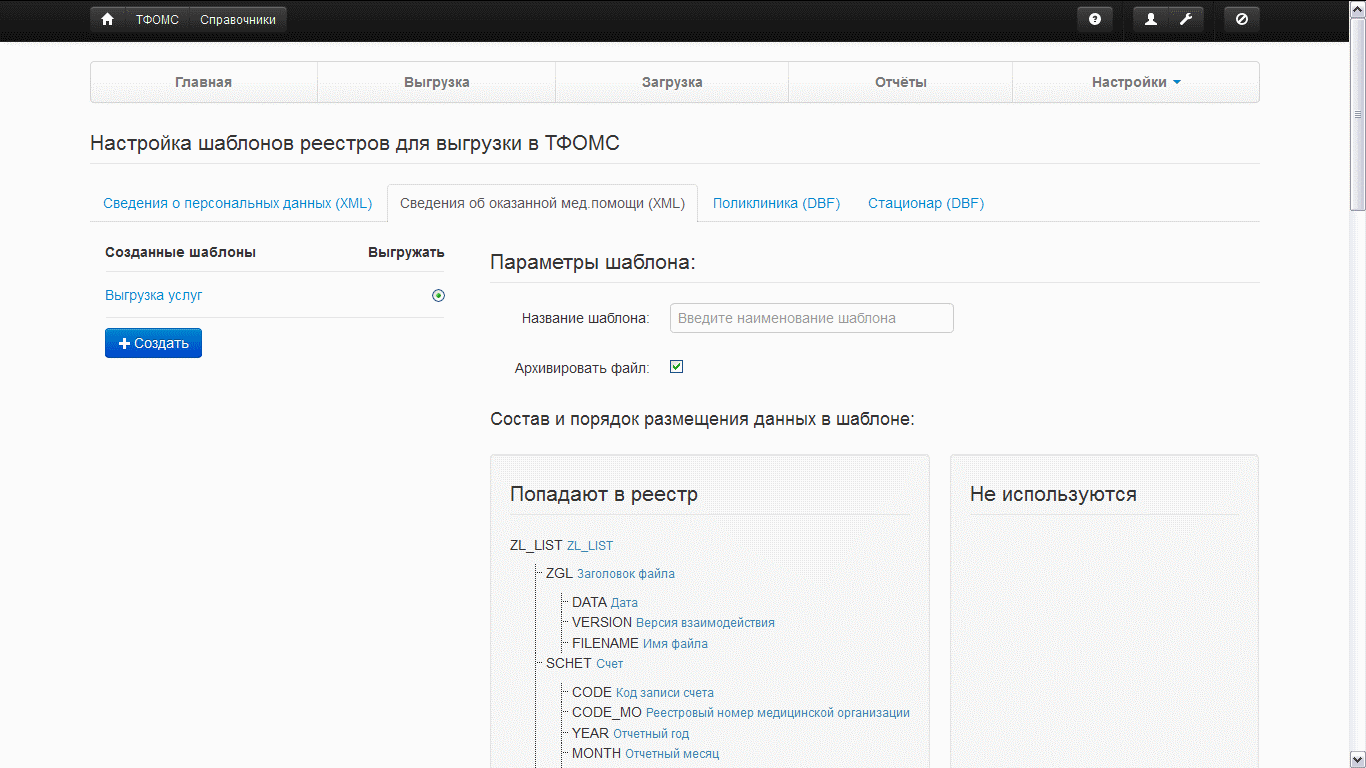
\includegraphics[width = 1\textwidth ,keepaspectratio]{tfoms_unload_conf2}
 \caption{Настройка шаблона выгрузки сведений об оказанных услугах}
 \label{img_tfoms_unload_conf2}
\end{figure}

Подробное описание допустимых полей для выгрузки приведено в таблице \ref{tbl_tfoms_srv_xml}.

\small{
\begin{longtable}{|p{2.1cm}|p{2.6cm}|p{2cm}|p{5cm}|p{4cm}|}
\caption{Состав полей для выгрузки сведений об оказанных услугах в XML \label{tbl_tfoms_srv_xml}}\\
\hline \rule{0pt}{15pt} \centering \textbf{Код элемента} & \centering \textbf{Наимено\-ва\-ние элемента} & \centering \textbf{Формат}  & \centering \textbf{Описание элемента} & \hfil \textbf{Поле в БД} \\ \hline
\endfirsthead
\hline \rule{0pt}{15pt} \centering \textbf{Код элемента} & \centering \textbf{Наимено\-ва\-ние элемента} & \centering \textbf{Формат}  & \centering \textbf{Описание элемента} & \hfil \textbf{Поле в БД} \\ \hline
\endhead
ZL\_LIST &	ZL\_LIST &	Составной элемент	& Корневой элемент  &  \\ \hline	
ZGLV &	Заголовок файла	& Составной элемент &	Элемент содержит общую информацию о файле выгрузки. Добавляется в начало файла 1 раз	&  \\ \hline
VERSION	& Версия взаимодействия	& Текст, 5 & 	Версия протокола взаимодействия, всегда ставится <<1.0>> &  \\ \hline	
DATA	& Дата	& Дата	& Дата формирования реестра в формате ГГГГ-ММ-ДД &  \\ \hline	
FILENAME	& Имя файла	& Текст, 26	& Имя текущего файла без расширения	&  \\ \hline
SCHET	& Счет	& Составной элемент	& Элемент содержит информацию о выставленном счете, переданном совместно с файлом выгрузки. Элементы добавляется в XML-файл сразу после заголовка. Количество элементов соответствует количеству выставленных счетов &  \\ \hline	
CODE	& Код записи счета	& Число, 8	& Порядковый номер счета в файле выгрузки (нумерация начинается с 1) &  \\ \hline	
CODE\_MO	& Реестровый номер медицинской организации	& Текст, 6 & 	Указывается в настройках Системы администрирования ЛПУ в поле \dm{ИНФИС код ЛПУ} (см. раздел \ref{gen_conf}) &  \\ \hline
YEAR	& Отчетный год	& Число, 4	& Подставляется год, за который формируется отчет &  \\ \hline	
MONTH	& Отчетный месяц	& Число, 2	& Подставляется номер месяца, за который формируется отчет &  \\ \hline	
NSCHET	& Номер счета	& Текст, 15	& Формируется номер счета следующего формата ГГММ-N/ Ni,
Где N = 1 для основного счета, N = 2 для дополнительного счета
Ni = первые 3 цифры кода ЛПУ. 
Код ЛПУ указывается в настройках Системы администрирования ЛПУ в поле \dm{Старый ИНФИС код ЛПУ} (см. раздел \ref{gen_conf}) &  \\ \hline
DSCHET	& Дата выставления счета	& Дата	& Указывается текущая дата на момент формирования файла в формате ГГГГ-ММ-ДД &  \\ \hline	
PLAT	& Плательщик. Реестровый номер СМО	& Текст, 5	& Указывается <<58000>> &  \\ \hline	
SUMMAV	& Сумма МО, выставленная на оплату & 	Число, 15,2	& Общая сумма, выставленная в файле к оплате &  \\ \hline	
COMENTS	& Служебное поле к счету	& Текст, 250 & 	Не заполняется &  \\ \hline	
SUMMAP	& Сумма, принятая к оплате СМО (ТФОМС) & Число, 15,2 & 	Не заполняется &  \\ \hline	
SANK\_MEK	& Финансовые санкции (МЭК)	& Число, 15,2 & Не заполняется &  \\ \hline	
SANK\_MEE	& Финансовые санкции (МЭЭ) &	Число, 15,2	& Не заполняется &  \\ \hline	
SANK\_EKMP & Финансовые санкции (ЭКМП)	& Число, 15,2 & Не заполняется &  \\ \hline	
ZAP	& Записи	& Составной элемент	& Записи о случаях оказания медицинской помощи &  \\ \hline	
N\_ZAP & Номер позиции записи	& Число, 8	& Порядковый номер записи в файле выгрузки (нумерация начинается с 1) &  \\ \hline	
PR\_NOV	& Признак исправленной записи	& Число, 1	& <<0>> – если сведения об оказанной медицинской помощи передаются впервые(основной счет). Для первого дополнительного счета (номер пакета N = 2) должен выгружаться признак <<1>>, для последующих (номер пакета N >= 3) - признак <<2>>. &  \\ \hline	
PACIENT	& Сведения о пациенте	& Составной элемент	& Данный тег выгружается 1 раз для каждого пациента, которому была оказана одна или более услуг за отчетный период	&  \\ \hline
ID\_PAC	& Код записи о пациенте	& Текст, 36	& Указывается код регистрационной карточки пациента. В некоторых случаях необходимо выгружать по одному пациенту несколько записей с разными значениями <ID\_PAC>; в этом случае в теге <ID\_PAC> выгружается порядковый номер пациентов (начина с 1 и далее) & 	Client.id  \\ \hline
VPOLIS	& Тип документа, подтверждающего факт страхования по ОМС &	Число, 1	& Выбирается из регистрационной карточки пациента в ФТМИС, со вкладки \dm{Паспортные данные}, поле \dm{СМО} (справа) в разделе \dm{Полис ОМС}. Типы полисов настраиваются в справочнике \mm{Справочники \str Персонификация \str Тип полиса} в поле \dm{Код}	& rbPolicyType.code. 
Необходимо для заданного пациента найти полис в таблице ClientPolicy, где 
ClientPolicy.deleted = 0 и  в записи о типе полиса rbPolicyType значение поля name начинается с <<ОМС>>  \\ \hline
SPOLIS	& Серия документа, подтверждающего факт страхования по ОМС	& Текст, 10	& Выбирается из регистрационной карточки пациента в ФТМИС, со вкладки \dm{Паспортные данные}, поле \dm{Серия} в разделе \dm{Полис ОМС}. &	ClientPolicy.serial
для записи ClientPolicy, найденной в предыдущем теге (VPOLIS) \\ \hline
NPOLIS	& Номер документа, подтверждающего факт страхования по ОМС	& Текст, 20	& Выбирается из регистрационной карточки пациента в ФТМИС, со вкладки \dm{Паспортные данные}, поле \dm{Номер} в разделе \dm{Полис ОМС}. &	ClientPolicy.number
для записи ClientPolicy, найденной в теге (VPOLIS)  \\ \hline
SMO	& Реестровый номер СМО	& Текст, 5	& Выбирается из регистрационной карточки пациента в ФТМИС, со вкладки \dm{Паспортные данные}, поле \dm{СМО} (слева) в разделе \dm{Полис ОМС}. 
Номер СМО задается в справочнике организаций (\mm{Справочники \str Организации \str Организации}) в поле ИНФИС &	Organization.infisCode
для записи ClientPolicy, найденной в теге (VPOLIS)  \\ \hline
SMO\_OGRN	& ОГРН СМО	& Текст, 15	& Не заполняется &  \\ \hline	
SMO\_OK	& ОКАТО территории страхования &	Текст, 5 & 	&  \\ \hline	
SMO\_NAM	& Наименование СМО	& Текст, 100 &	Не заполняется &  \\ \hline	
SLUCH	& Сведения о случае	& Составной элемент & &  \\ \hline		
IDCASE	& Номер записи в реестре случаев	& Число, 8 &	Выгружается внутренний идентификатор позиции счета. В дальнейшем будет использоваться для проставления признака подтверждения оплаты или отказа от ТФОМС	& Account\_Item.id  \\ \hline
USL\_OK	& Условия оказания медицинской помощи	& Число, 2 & 	Настройка соответствия типа события и его назначения производится в карточке типа события, поле \dm{Назначение}. Назначения типов событий настраиваются в справочнике \mm{Справочники \str Учет \str Назначение типа события} &	rbEventTypePurpose. code \\ \hline
VIDPOM	& Вид помощи	& Число, 4	& Настройка соответствия типа события и вида помощи производится в карточке типа события, поле \dm{Тип медицинской помощи}. Виды помощи настраиваются в справочнике \mm{Справочники \str Учет \str Типы медицинской помощи}	& rbMedicalAidType. code  \\ \hline
NPR\_MO	& Код МО, направившего на лечение (госпитализацию, диагностику, консультацию)	& Текст, 6	& Не заполняется &  \\ \hline	
EXTR &	Направление (госпитализации)	& Число, 2	& <<1>> – плановая, <<2>> – экстренная.
Если в поле \dm{Порядок} карточки обращения указано <<экстренно>>, то обращение считается экстренным. При значениях данного поля обращение считается плановым &	Если Event.order = 2, то <<2>>
иначе <<1>>  \\ \hline
LPU	& Код МО	& Текст, 6	& Указывается в настройках Системы администрирования ЛПУ в поле \dm{ИНФИС код ЛПУ} (см. раздел \ref{gen_conf}) &  \\ \hline
LPU\_1	& Подразделение МО	& Текст, 6	& Указывается в настройках Системы администрирования ЛПУ в поле \dm{Старый ИНФИС код ЛПУ} (см. раздел \ref{gen_conf}) & \\ \hline
PODR &	Код отделения	& Число, 8	& В случае поликлиники выбирается соответствующее действие <<Осмотр/консультация>> в разделе \dm{Медицинские документы} карточки обращения и определяется тип действия выбранной услуги из справочника \mm{Справочники \str Учет \str Типы действий}. В карточке типа действия на вкладке \dm{Оплата/Квотирование} в поле \dm{Услуга} по умолчанию указана соответствующая услуга.
В случае стационара выбирается действие <<Движение>> в разделе \dm{Движение пациента} карточки обращения, в котором получаем значение свойства <<Профиль койки>>. Профили койки настраиваются в справочнике \mm{Справочники \str Учет \str Профили коек}. В карточке профиля койки на вкладке \dm{Услуги} необходимо выбрать услугу соответствующую типу стационара и возрасту пациента.
В справочнике услуг \mm{Справочники \str Финансовые \str Услуги (профиль ЕИС)} в поле  & rbService.departCode \\ \hline
 & & & \dm{Код отделения} указывается соответствующий код подразделения & \\ \hline
PROFIL	& Профиль	& Число, 3	& Задается в карточке услуги на вкладке \dm{Профили по умолчанию}.
Настройка доступных профилей производится в справочнике \mm{Справочники \str Учет \str Профили медицинской помощи} &	rbMedicalAidProfile. code  \\ \hline
DET	& Признак детского профиля	& Число, 1	& <<0>> - нет, <<1>> - да. Если возраст пациента меньше 18 лет, то выставляется <<1>>. Во всех остальных случаях – <<0>>	& Вычисляется на основании поля Client.birthDate \\ \hline
NOVOR	& Признак новорождённого	& Текст, 9	& Указывается в случае оказания медицинской помощи ребёнку до получения им собственного полиса.
Если признак отсутствует, то ставится <<0>>, иначе заполняется по шаблону 
ПДДММГГН, где П – пол ребенка, ДД – день рождения, ММ – месяц рождения, ГГ – последние 2 цифры года рождения, Н – порядковый номер ребенка при многоплодных родах.
Пациент считается новорожденным до 28 дней.
Пол и возраст пациента подставляются из соответствующих полей регистрационной карточки пациента. Номер ребенка хранится в регистрационной карточке пациента на вкладке \dm{Прочее} для типа записи <<Номер ребенка при многоплодных родах>> & 	Client.birthDate,
Client.sex, 
ClientContact.contact, такая что 
ClientContact.Contact\-Type\_id ссылается на идентификатор записи rbContactType, в которой  значение поля name = <<Номер ребенка при многоплодных родах>> \\ \hline
NHISTORY	& Номер истории болезни/ талона амбулаторного пациента/амбулаторная карта & Текст, 50 & Для поликлиники: если в свойствах действия, заполняемых на форме обращения, присутствует свойство с названием <<Номер исследования для ТФОМС>>, то необходимо взять его значение. Если значение пустое или свойство отсутствует в действии, необходимо указать код регистрационной карточки пациента. 
Для стационара: если в типе события настроен внешний идентификатор (счетчик), то выгручается его значение. Если нет внешнего идентификатора – выгружается значение свойства с названием <<Номер ИБ>> (или <<Номер ИР>>) из действия <<Поступление>>, созданного в рамках текущего обращения	& ActionProperty\_ String.value, где ActionProperty.type\_ id, ссылается на идентификатор id записи ActionPropertyType с полем name = <<Номер исследования для ТФОМС>>.
Client.id – код регистрационной карты пациента; Event.externalId – внешний идентификатор; ActionProperty\_ String.value – значение свойства, связанное с ActionPropertyType, где ActionPropertyType. name = <<Номер ИБ>> или <<Номер ИР>> \\ \hline
DATE\_1	& Дата начала лечения	& Дата	& Значение поля \dm{Начато} карточки действия	& Action.begDate \\ \hline
DATE\_2	& Дата окончания лечения	& Дата	& Значение поля \dm{Выполнено} карточки действия	& Action.endDate \\ \hline
DS0	& Диагноз первичный (код клинической стадии онкологического заболевания)	& Текст, 10	& Проставляется код, соответствующий значению, указанному в поле \dm{Фаза заболевания} заключительного диагноза, указанного в таблице диагнозов, открывающейся после нажатия кнопки  \btn{Окончательные диагнозы} в карточке обращения.
Фазы заболевания настраиваются в справочнике \mm{Справочники \str Медицинские \str Фазы заболевания} &	rbDiseasePhases.code \\ \hline
DS1	& Диагноз основной	& Текст, 10	& Проставляется значение поля \dm{МКБ} заключительного диагноза указанного в таблице диагнозов, открывающейся после нажатия кнопки  \btn{Окончательные диагнозы} в карточке обращения	& Diagnosis.MKB \\ \hline
DS2	& Диагноз сопутствующего заболевания	& Текст, 10 & 	Проставляется значение поля \dm{МКБ} сопутствующего диагноза указанного в таблице диагнозов, открывающейся после нажатия кнопки  \btn{Окончательные диагнозы} в карточке обращения &	Diagnosis.MKB \\ \hline
CODE\_MES1	& Код МЭС	& Текст, 16	& Не заполняется &  \\ \hline	
CODE\_MES2	& Код МЭС сопутствующего заболевания	& Текст, 16	& Не заполняется	&  \\ \hline
RSLT	& Результат обращения/ госпитализации & 	Число, 3	& Проставляется код, соответствующий значению, указанному в поле Результат основного диагноза в карточке обращения пациента.	& rbResult.code \\ \hline
ISHOD	& Исход заболевания	& Число, 3	& Выгружается код соответствующий значению, выбранному в поле \dm{Исход госпитализации} (стационар) или \dm{Исход заболевания} (поликлиника). Исходы заболеваний настраивается в справочнике \mm{Справочники \str Медицинские \str Исходы заболеваний}	& rbAcheResult.code \\ \hline
PRVS	 &Специальность лечащего врача/ врача, закрывшего талон & 	Число, 9	& В случае поликлиники выбирается соответствующее действие <<Осмотр/консультация>> в разделе \dm{Медицинские документы} карточки обращения, в поле \dm{Исполнитель} указан врач, закрывший талон. В случае стационара выбирается последнее действие <<Движение>> в разделе \dm{Движение пациента} карточки обращения, в поле \dm{Исполнитель} указан врач, закрывший действие. 
Выгружается код специальности врача, являющегося исполнителем в указанном действии. Коды специальностей настраиваются в справочнике \mm{Справочники \str Персонал \str Специальности} в поле \dm{Код}	& rbSpeciality.code \\ \hline
IDDOKT	& СНИЛС врача, закрывшего талон/историю болезни	& Текст, 16	& В случае поликлиники выбирается соответствующее действие <<Осмотр/консультация>> в разделе \dm{Медицинские документы} карточки обращения, в поле \dm{Исполнитель} указан врач, закрывший талон. В случае стационара выбирается последнее действие <<Движение>> в разделе \dm{Движение пациента} карточки обращения, в поле \dm{Исполнитель} указан врач, закрывший действие. Выгружается СНИЛС врача, являющегося исполнителем в указанном действии. СНИЛС выгружается в виде строки с разделителями, в формате <<999-999-999 99>>. СНИЛС врача указывается в карточке сотрудника \mm{Справочники \str Персонал \str Сотрудники} в поле \dm{СНИЛС} & Person.SNILS \\ \hline
OS\_SLUCH	& Признак <<Особый случай>> при регистрации обращения за медицинской помощью	& Число, 1	& <<1>> - медицинская помощь оказана новорожденному ребенку до государственной регистрации рождения при многоплодных родах; <<2>> – в документе, удостоверяющем личность пациента/родителя (представителя) пациента, отсутствует отчество. <<1>> указывается, если помощь оказана ребенку в возрасте до 28 дней и на вкладке \dm{Прочее} регистрационной карточки пациента присутствует строка <<Номер ребенка при многоплодных родах>> с заполненным номером. <<2>> ставится, если не задано отчество пациента и не задан представитель. Либо в регистрационной карточке представителя не указано отчество. Представитель указывается на вкладке \dm{Связи} регистрационной карточки пациента в таблице Обратная связь &	<<1>> ставится, если существует запись ClientContact, где ContactType\_id, соответствует записи rbContactType, в которой  значение поля name = <<Номер ребенка при многоплодных родах>>.
<<2>> ставится, если не заполнено поле Client.patrName в записи о пациенте (если нет представителя) или в записи о представителе (если есть представитель) \\ \hline
IDSP	& Код способа оплаты медицинской помощи	& Число, 2	& В случае поликлиники выбирается соответствующее действие <<Осмотр/консультация>> в разделе \dm{Медицинские документы} карточки обращения и определяется тип действия выбранной услуги из справочника \mm{Справочники \str Учет \str Типы действий}. В карточке типа действия на вкладке \dm{Оплата/Квотирование} в поле \dm{Услуга по умолчанию} указана соответствующая услуга. В случае стационара выбирается действие <<Движение>> в разделе \dm{Движение пациента} карточки обращения, в котором получаем значение свойства <<Профиль койки>>. Профили койки настраиваются в справочнике \mm{Справочники \str Учет \str Профили коек}. В карточке профиля койки на вкладке \dm{Услуги} необходимо выбрать услугу, соответствующую типу стационара и возрасту пациента. В справочнике услуг \mm{Справочники \str Финансовые \str Услуги (профиль ЕИС)} в поле \dm{Категория} указывается категория медицинской помощи. В справочнике \mm{Справочники \str Учет \str Связь категории помощи и способа оплаты услуг} выбирается значение поля \dm{Способ оплаты}, соответствующее типу события и найденной категории помощи. Выгружается код, соответствующий указанному способу оплаты. Коды способов оплаты настраиваются в справочнике \mm{Справочники  Финансовые \str Способы оплаты}. В случае стационарного обращения, код способа оплаты зависит так же от количества койко-дней, проведенных в стационаре &	rbPayType.code  \\ \hline
ED\_COL	& Количество единиц оплаты медицинской помощи &	Число, 5, 2 &	Для поликлиники (кроме стоматологии) = 1. Для стоматологии = число УЕТ, соответствующих одной услуге. Если было оказано несколько одинаковых услуг, то каждая услуга выводится отдельным тегом <SLUCH>. Но в рамках каждого <SLUCH> (и каждого <USL> внутри него) выводится количество УЕТ, соответствующее одной услуге. Для круглосуточного стационара = 1 (если дата начала действия <<Движение>> совпадает с датой окончания). Иначе - разница между датой окончания и датой начала <<Движения>>. Для дневного стационара = 1 (если дата начала действия <<Движение>> совпадает с датой окончания). Иначе - разница между датой окончания и датой начала <<Движения>> плюс один день и минус число воскресений, попавших в период лечения. &	Contract\_Tariff.uet – для стоматологии. Для стационара и дневного стационара: Action.begDate, Action.endDate  \\ \hline
TARIF	& Тариф	& Число, 15, 2	& Не заполняется &  \\ \hline	
SUMV	& Сумма, выставленная к оплате	& Число, 15, 2 & Складываются значения полей SUMV\_USL из тегов USL внутри текущего тега SLUCH &  \\ \hline	
OPLATA	& Тип оплаты	& Число, 1	& Заполняется СМО(ТФОМС) &  \\ \hline	
SUMP	& Сумма, принятая к оплате СМО (ТФОМС)	& Число, 15, 2 & 	Заполняется СМО(ТФОМС) &  \\ \hline	
REFREA-SON	& Код причины отказа (частичной) оплаты	& Число, 2 & 	Заполняется СМО(ТФОМС)	& rbPayRefuseType.code. Сохраняется в поле Account\_Item.refuse Type\_id при загрузке данных из ТФОМС. Кроме того, в поле Account\_Item.date сохраняется текущая дата, в поле  Account\_Item.number – название файла  \\ \hline
SANK\_ MEK	& Финансовые санкции (МЭК)	& Число, 15, 2 & &  \\ \hline		
SANK\_ MEE	& Финансовые санкции (МЭЭ)	 & Число, 15, 2 & &  \\ \hline		
SANK\_ EKMP	& Финансовые санкции (ЭКМП)	& Число, 15, 2 & &  \\ \hline		
USL	& Сведения об услуге	& Составной элемент & &  \\ \hline		
IDSERV	& Номер записи в реестре услуг	& Число, 8	& Порядковый номер тега <USL> внутри тега <SLUCH>. При закрытии тега <SLUCH> обнуляется &  \\ \hline	
LPU	& Код МО	& Текст, 6	& Указывается в настройках Системы администрирования ЛПУ в поле \dm{ИНФИС код ЛПУ} (см. раздел \ref{gen_conf}) &  \\ \hline
LPU\_1	& Подразделение МО	& Текст, 6	& Указывается в настройках Системы администрирования ЛПУ в поле \dm{Старый ИНФИС код ЛПУ}  (см. раздел \ref{gen_conf}) &  \\ \hline
PODR	& Код отделения	& Число, 8	& В случае поликлиники выбирается соответствующее действие <<Осмотр/консультация>> в разделе \dm{Медицинские документы} карточки обращения и определяется тип действия выбранной услуги из справочника \mm{Справочники \str Учет \str Типы действий}. В карточке типа действия на вкладке \dm{Оплата/Квотирование} в поле \dm{Услуга по умолчанию} указана соответствующая услуга. В случае стационара выбирается действие <<Движение>> в разделе \dm{Движение пациента} карточки обращения, в котором получаем значение свойства <<Профиль койки>>. Профили койки настраиваются в справочнике \mm{Справочники \str Учет \str Профили коек}. В карточке профиля койки на вкладке \dm{Услуги} необходимо выбрать услугу соответствующую типу стационара и возрасту пациента. В справочнике услуг \mm{Справочники \str Финансовые \str Услуги (профиль ЕИС)} в поле & 	rbService.departCode  \\ \hline
 & & & \dm{Код отделения} указывается соответствующий код подразделения &   \\ \hline
PROFIL	& Профиль	& Число, 3	& Задается в карточке услуги на вкладке \dm{Профили по умолчанию}. Настройка доступных профилей производится в справочнике \mm{Справочники \str Учет \str Профили медицинской помощи}	& rbMedicalAidProfile. code  \\ \hline
DET	& Признак детского профиля	& Число, 1	& <<0>> - нет, <<1>> - да. Если возраст пациента меньше 18 лет, то выставляется <<1>>. Во всех остальных случаях – <<0>>	& Вычисляется на основании поля Client.birthDate \\ \hline
DATE\_IN	& Дата начала оказания услуги	& Дата	& В карточке обращения таблица \dm{Мероприятия}, значение столбца \dm{Начато} & Action.begDate  \\ \hline
DATE\_ OUT	& Дата окончания оказания услуги	& Дата	& В карточке обращения таблица \dm{Мероприятия}, значение столбца \dm{Окончено} &	Action.endDate \\ \hline
DS &	Диагноз	& Текст, 10	& Значение поля \dm{МКБ} диагноза карточки обращения	&  \\ \hline
CODE\_USL	& Код услуги	& Текст, 16	& Код услуги формируется в соответствии с требованиями ТФОМС региона &  \\ \hline	
KOL\_USL	& Количество услуг (кратность услуги)	& Число, 6, 2 & 	Для поликлиники (кроме стоматологии) = 1. Для стоматологии = число УЕТ, соответствующих одной услуге. Если было оказано несколько одинаковых услуг, то каждая услуга выводится отдельным тегом <SLUCH>. Но в рамках каждого <SLUCH> (и каждого <USL> внутри него) выводится количество УЕТ, соответствующее одной услуге. Для круглосуточного стационара = 1 (если дата начала действия <<Движение>> совпадает с датой окончания). Иначе - разница между датой окончания и датой начала <<Движения>>. Для дневного стационара = 1 (если дата начала действия <<Движение>> совпадает с датой окончания). Иначе - разница между датой окончания и датой начала <<Движения>> плюс один день и минус число воскресений, попавших в период лечения.	& Contract\_Tariff.uet – для стоматологии. Для стационара и дневного стационара: Action.begDate, Action.endDate  \\ \hline
TARIF	& Тариф	& Число, 15, 2	& В пункте меню \mm{Расчет \str Договоры} выбирается договор <<ОМС>>. Для выбранного договора на вкладке \dm{Тарифы} необходимо выбрать тариф в соответствии с выполненным осмотром или профилем койки, возрастом пациента, в некоторых случаях учитываются так же пол и тип события. Необходимо выбрать действующий тариф (где в полях \dm{Дата начала} и \dm{Дата окончания} указан период, в который попадает период выгрузки). В случае оплаты в стационаре по стандартам выбор производится не по услуге, а по коду диагноза МКБ (столбец \dm{Код по МКБ}).  На одну услугу (один диагноз МКБ). Соответственно, каждая такая запись будет выводиться отдельным тегом <USL> (в рамках тега <SLUCH>).
В случае оплаты по УЕТ (на данный момент только стоматология) цену тарифа необходимо разделить на число УЕТ, соответствующих одной услуге, чтоб получить цену одного УЕТ &	Contract\_Tariff.price \\ \hline
SUMV\_ USL	& Стоимость медицинской услуги, выставленная к оплате (руб.)	& Число, 15, 2	& В карточке обращения на вкладке \dm{Оплата}, на вкладке \dm{Услуги} значение поля \dm{Сумма} в таблице \dm{Оказанные услуги} & Значение поля <<TARIF>> умножается на значение поля <<KOL\_USL>> в текущем теге \\ \hline
PRVS	& Специальность медработника, выполнившего услугу	& Число, 9	& В случае поликлиники выбирается соответствующее действие <<Осмотр/консультация>> в разделе \dm{Медицинские документы} карточки обращения, в поле \dm{Исполнитель} указан врач, закрывший талон. В случае стационара выбирается последнее действие <<Движение>> в разделе \dm{Движение пациента} карточки обращения, в поле \dm{Исполнитель} указан врач, закрывший действие. Выгружается код специальности врача, являющегося исполнителем в указанном действии. Коды специальностей настраиваются в справочнике \mm{Справочники \str Персонал \str Специальности} в поле \dm{Код}	& rbSpeciality.code \\ \hline
CODE\_MD	& Код медицинского работника, оказавшего медицинскую услугу	& Текст, 16	& В случае поликлиники выбирается соответствующее действие <<Осмотр/консультация>> в разделе \dm{Медицинские документы} карточки обращения, в поле \dm{Исполнитель} указан врач, закрывший талон. В случае стационара выбирается последнее действие <<Движение>> в разделе \dm{Движение пациента} карточки обращения, в поле \dm{Исполнитель} указан врач, закрывший действие. Выгружается СНИЛС врача, являющегося исполнителем в указанном действии. СНИЛС выгружается в виде строки с разделителями, в формате <<999-999-999 99>>. СНИЛС врача указывается в карточке сотрудника \mm{Справочники \str Персонал \str Сотрудники} в поле \dm{СНИЛС} &	Person.SNILS \\ \hline
COMENTU	& Служебное поле	& Текст, 250	& &  \\ \hline	
COMENTSL	& Служебное поле	& Текст, 250 &	Заполняется СМО(ТФОМС). Содержит пояснения по причине отказа &	Сохраняется в Account\_Item.note при загрузке данных из ТФОМС \\ \hline
\end{longtable}
}

\subsubsection{Настройка выгрузки сведений об оказанных поликлинических услугах в формате DBF}

Для настройки данного типа шаблона необходимо перейти на вкладку Поликлиника (DBF) (Рисунок \ref{img_tfoms_unload_conf3}). Подробное описание допустимых полей для выгрузки приведено в таблице \ref{tbl_tfoms_pol_dbf}.

\begin{figure}[ht]\centering
 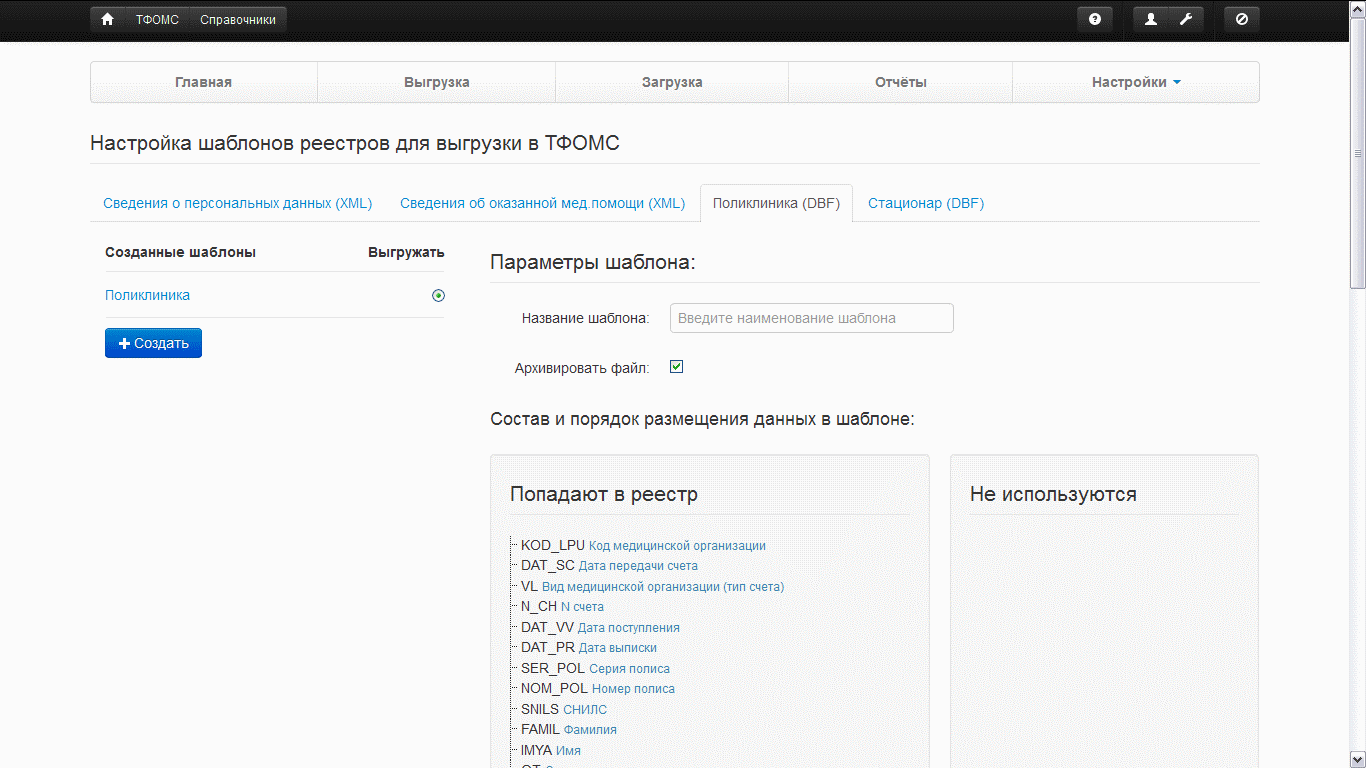
\includegraphics[width = 1\textwidth ,keepaspectratio]{tfoms_unload_conf3}
 \caption{Настройка шаблона выгрузки сведений об оказанных в поликлинике услугах в формате DBF}
 \label{img_tfoms_unload_conf3}
\end{figure}

\small{
\begin{longtable}{|p{2.1cm}|p{2.6cm}|p{2cm}|p{5cm}|p{4cm}|}
\caption{Состав полей для выгрузки сведений об оказанных в поликлинике услугах в формате DBF \label{tbl_tfoms_pol_dbf}}\\
\hline \rule{0pt}{15pt} \centering \textbf{Код элемента} & \centering \textbf{Наимено\-ва\-ние элемента} & \centering \textbf{Формат}  & \centering \textbf{Описание элемента} & \hfil \textbf{Поле в БД} \\ \hline
\endfirsthead
\hline \rule{0pt}{15pt} \centering \textbf{Код элемента} & \centering \textbf{Наимено\-ва\-ние элемента} & \centering \textbf{Формат}  & \centering \textbf{Описание элемента} & \hfil \textbf{Поле в БД} \\ \hline
\endhead
KOD\_LPU & 	Код медицинской  организации	& numeric(3)	& Указывается в настройках Системы администрирования ЛПУ в поле \dm{ИНФИС код ЛПУ} (см. раздел \ref{gen_conf}) &  \\ \hline
DAT\_SC &	Дата передачи счета	& date(8)	& Дата формирования реестра	& Account.date \\ \hline
VL	& Вид медицинской  организации (тип счета)	& numeric(1)	& Устанавливается значение <<2>> &  \\ \hline	
N\_CH & 	N счета	& character (10)	& Номер счета &	Account.number \\ \hline
DAT\_VV & 	Дата начала лечения	& date & & \\ \hline		
DAT\_PR &	Дата окончания лечения	& date & &  \\ \hline		
SER\_POL	 & Серия полиса	& character(4)	& Выбирается из регистрационной карточки пациента в ФТМИС, со вкладки \dm{Паспортные данные}, поле \dm{Серия} в разделе \dm{Полис ОМС}. & ClientPolicy.serial для записи ClientPolicy, где 
ClientPolicy.deleted = 0 и  в записи о типе полиса rbPolicyType значение поля name начинается с <<ОМС>>  \\ \hline
NOM\_POL	& Номер полиса	& numeric(12)	& Выбирается из регистрационной карточки пациента в ФТМИС, со вкладки \dm{Паспортные данные}, поле \dm{Номер} в разделе \dm{Полис ОМС}. &	ClientPolicy.number для записи ClientPolicy, где 
ClientPolicy.deleted = 0 и  в записи о типе полиса rbPolicyType значение поля name начинается с <<ОМС>> \\ \hline
SNILS	& СНИЛС пациента	& character (14)	& Выбирается из регистрационной карточки пациента в ФТМИС, поле \dm{СНИЛС}	& Client.SNILS \\ \hline
FAMIL 	& Фамилия	& character (12)	& Выбирается из регистрационной карточки пациента в ФТМИС, поле \dm{Фамилия}	& Client.lastName \\ \hline
IMYA	& Имя	& character (15)	& Выбирается из регистрационной карточки пациента в ФТМИС, поле \dm{Имя}	& Client.firstName  \\ \hline
OT	& Отчество & character (15)	& Выбирается из регистрационной карточки пациента в ФТМИС, поле \dm{Отчество} &	Client.patrName \\ \hline
KOD\_F &	Код страховой компании	& numeric(4) &	Выбирается из регистрационной карточки пациента в ФТМИС, со вкладки \dm{Паспортные данные}, поле \dm{СМО} (слева) в разделе \dm{Полис ОМС}. Номер СМО задается в справочнике организаций (\mm{Справочники \str Организации \str Организации}) в \dm{поле ИНФИС} &	Organization.infisCode
для записи ClientPolicy, где ClientPolicy.deleted = 0 и  в записи о типе полиса rbPolicyType значение поля name начинается с <<ОМС>>  \\ \hline
POL	& Пол	& character(1)	& Выбирается из регистрационной карточки пациента в ФТМИС, поле \dm{Пол}.	& Client.sex  \\ \hline
D\_R & 	Дата рождения &	date	& Выбирается из регистрационной карточки пациента в ФТМИС, поле \dm{Д.рожд.}	& Client.birthDate  \\ \hline
RAION	& Район	& numeric(2)	& Используется региональный справочник кодов районов.Справочник заливается в таблицу rbDistrict64 &	rbDistrict64.infis. Определить первые 2 символа кода КЛАДР адреса проживания. В таблице rbDistrict64 найти запись, в которой parent пусто и prefix равняется этим двум символам.  \\ \hline
KOD\_T	& Код территории РФ	& numeric(4)	& Используется региональный справочник кодов территорий. Справочник заливается в таблицу rbDistrict64	& rbDistrict64.infis. Определить первые 10 символов кода КЛАДР улицы адреса проживания. Добавляем в конец полученного значения <<000>>. В результате получаем код КЛАДР района проживания, по нему в таблице rbDistrict64 ищем запись  \\ \hline
NAS\_P	& Населенный пункт	& character(30)	& Выбирается из регистрационной карточки пациента в ФТМИС, поле \dm{Адрес регистрации}.	& Kladr.KLADR.Name  \\ \hline
UL	& Улица	& character(20)	& Выбирается из регистрационной карточки пациента в ФТМИС, поле \dm{Адрес регистрации}.	& Kladr.KLADR.Name  \\ \hline
DOM	& Дом	& character(6)	& Выбирается из регистрационной карточки пациента в ФТМИС, в подразделе \dm{Адрес регистрации} значение поля \dm{Дом} &	AddressHouse. Numericber  \\ \hline
KV	& Квартира	& character(4)	& Выбирается из регистрационной карточки пациента в ФТМИС, в подразделе \dm{Адрес регистрации} значение поля \dm{Квартира} & 	Address.flat  \\ \hline
KATEGOR	& Категория	& numeric(1) &	<<1>> - работающий, <<2>> - неработающий &   \\ \hline	
MES\_R & 	Место работы	& character (80) & &   \\ \hline		
KOD\_PR	& Регистрационный номер предприятия	& character (15) &	Не заполняется	&   \\ \hline
OTD	& Код отделения стационара	& numeric(3) &	Ищется услуга, соответствующая типу действия. В карточке услуги указывается код отделения в поле \dm{Отделение} & 	rbService.departCode  \\ \hline
N\_KART	& N истории болезни или N карты	& character(8) & &   \\ \hline		
KC	& Цель обращения	& numeric(2)	& Поле \dm{Код} в карточке соответствующего события	& EventType.Code  \\ \hline
DIA\_O	& Диагноз основной	& character(6)	& Указывается значение поля \dm{МКБ} для основного диагноза в таблице диагнозов карточки обращения	& Diagnosis.MKB  \\ \hline
DOP\_D	& Дополнение к основ. диагнозу	& character (80) &	Подставляется описание для кода МКБ, указанного выше из справочника \dm{Справочники \str Медицинские \str Коды МКБ Х} &	MKB. DiagID  \\ \hline
DIA\_S &	Диагноз сопутствующий 1	& character(6) & 	Указывается значение поля МКБ для первого найденного сопутствующего диагноза в таблице диагнозов карточки обращения	& Diagnosis.MKB  \\ \hline
DOP\_S	& Дополнение к сопутствующему  диагнозу 1	& character (80)	& Подставляется описание для кода МКБ, указанного выше из справочника \mm{Справочники \str Медицинские \str Коды МКБ Х} & 	MKB. DiagID  \\ \hline
DIA\_S1	& Диагноз сопутствующий 2	& character(6) & 	Указывается значение поля МКБ для второго найденного сопутствующего диагноза в таблице диагнозов карточки обращения	& Diagnosis.MKB  \\ \hline
DOP\_S1	& Дополнение к сопутствующему  диагнозу 2 & 	character (80)	& Подставляется описание для кода МКБ, указанного выше из справочника \mm{Справочники \str Медицинские \str Коды МКБ Х} & MKB. DiagID  \\ \hline
OSL	& Диагноз осложнения	& character(6) & Указывается значение поля \dm{МКБ} для второго найденного диагноза осложнения в таблице диагнозов карточки обращения &	Diagnosis.MKB  \\ \hline
DOP\_OSL	& Дополнение к диагнозу осложнения &  	character (80)	& Подставляется описание для кода МКБ, указанного выше из справочника \mm{Справочники \str Медицинские \str Коды МКБ Х} &	MKB. DiagID  \\ \hline
KSG\_MS &	Шифр МС	& character (20)	& Не заполняется &   \\ \hline	
DL\_LEC	& Продолжи\-тель\-ность лечения	& numeric(3) & &   \\ \hline		
KOL\_POS	& Количество посещений в поликлинике &   	numeric(2) & &   \\ \hline		
POS\_D	& Количество посещений на дому	& numeric(2) & &   \\ \hline		
SL	& Случай обслуживания	& numeric(1)	& Указывается значение поля \dm{Результат} для основного диагноза в таблице диагнозов карточки обращения	& rbResult.regionalcode  \\ \hline
ISH\_LEC	& Исход лечения	& numeric(2)	& Указывается значение поля \dm{Исход} для основного диагноза в таблице диагнозов карточки обращения	& rbArchResult.regional\-code  \\ \hline
PR\_NZ	& Причины незаконченности случая	& numeric(2) &	Указывается значение поля \dm{Хар} для основного диагноза в таблице диагнозов карточки обращения & rbDiseasecharacterac\-ter.Code  \\ \hline
STOIM	& Стоимость лечения	& numeric(13, 2)	& В карточке обращения на вкладке \dm{Оплата}, вкладке \dm{Услуги}, в таблице \dm{Оказанные услуги} в поле \dm{Цена} & 	Contract\_Tariff.price  \\ \hline
KOD\_VR	& Код лечащего врача	& character(6)	& Выгружается значение поля \dm{Код} в карточке сотрудника, указанного в поле \dm{Выполнил} соответствующего действия &  Person.code  \\ \hline
S\_VR & 	Специаль\-ность врача	& numeric(3)	& Выгружается код, соответствующей значению, выбранному в поле \dm{Должность} карточки сотрудника, указанного в поле \dm{Выполнил} соответствующего действия. Коды должностей задаются в справочнике \dm{Справочники \str Сотрудники \str Должности}	& rbPost.code  \\ \hline
NOM\_SL	& Номер случая обслуживания	& character (10)	& Не заполняется &   \\ \hline	
KOD\_O	& Код услуги, обследования, операции в  медицинской  организации	& character (10)	& Не заполняется &   \\ \hline	
N\_OPER	& Наимен. услуги, обследования, операции    & 	character (55)	& Не заполняется &   \\ \hline	
KOL\_USL	& Кол-во услуг и т.п	& numeric(3)	& Не заполняется &   \\ \hline	
KOD\_TSK & 	Код территории СМО	& numeric(4)	& По умолчанию = 0 &   \\ \hline	
NAMCMO	& Наименование СМО территории РФ	& character (40) & Выбирается из регистрационной карточки пациента в ФТМИС, со вкладки \dm{Паспортные данные}, поле \dm{СМО} (слева) в разделе \dm{Полис ОМС}. Номер СМО задается в справочнике организаций (\dm{Справочники \str Организации \str Организации}) в поле \dm{ИНФИС}	& Organization. shortName  \\ \hline
KOD\_DOK	& Вид документа	& numeric(2)	& Выбирается из регистрационной карточки пациента в ФТМИС, со вкладки \dm{Паспортные данные}, поле \dm{Документ}. Справочник типов документов настраивается в меню \mm{Справочники \str Персонификация \str Тип документа (паспорт и пр.)}, в поле \dm{Региональный код} следует указать код документа для выгрузки	& rbDocumentType. regionalCode. Ищется ClientDocument, такое что ClientDocument. deleted = 0 для заданного клиента, а затем из найденных записей выбирается такая, что rbDocumentType. group\_id = 1 (удостоверение личности)  \\ \hline
SER\_DOK	& Серия документа	& character (10)	& Выбирается из регистрационной карточки пациента в ФТМИС, со вкладки \dm{Паспортные данные}, поле \dm{Серия} в разделе \dm{Документ} &	ClientDocument.serial для записи, найденной в предыдущем поле (KOD\_DOK)  \\ \hline
NOM\_DOK	& Номер документа	& character (10)	& Выбирается из регистрационной карточки пациента в ФТМИС, со вкладки \dm{Паспортные данные}, поле \dm{Номер} в разделе \dm{Документ} &	ClientDocument. number для записи, найденной в поле (KOD\_DOK)  \\ \hline
VMP	& Вид мед.помощи	& numeric(2)	& Настройка соответствия типа события и вида помощи производится в карточке типа события, поле \dm{Тип медицинской помощи}. Виды помощи настраиваются в справочнике \mm{Справочники \str Учет \str Типы медицинской помощи} &	rbMedicalAidType. code  \\ \hline
DAT\_BLVN	& Дата выдачи листка временной нетрудоспособности & date &	Не заполняется &   \\ \hline	
DAT\_ELVN	& Дата закрытия листка временной нетрудоспособности	& date	& Не заполняется &  \\ \hline	
DAMAGE	& Признак травматизма на производстве	& numeric(1)	& Проставляется <<2>>, если в карточке обращения  в таблице \dm{Диагнозы} существует хотя бы 1 запись, с заполненным полем \dm{Травма} &	Diagnostic. traumaType\_id   \\ \hline
DATA\_NS	& Дата несчастного случая на   производстве & 	date	& Не заполняется  &  \\ \hline	
N\_NAPR	& N направления, направившее учреждение или отметка о приеме по ск.пом. &  & &   \\ \hline 			
\end{longtable}
}

\subsubsection{Настройка выгрузки сведений о лечении в стационаре в формате DBF}

Для настройки данного типа шаблона необходимо перейти на вкладку \dm{Стационар (DBF)}. Подробное описание допустимых полей для выгрузки приведено в таблице \ref{tbl_tfoms_st_dbf}.

\small{
\begin{longtable}{|p{2.1cm}|p{2.6cm}|p{2cm}|p{5cm}|p{4cm}|}
\caption{Состав полей для выгрузки сведений об оказанных в поликлинике услугах в формате DBF \label{tbl_tfoms_st_dbf}}\\
\hline \rule{0pt}{15pt} \centering \textbf{Код элемента} & \centering \textbf{Наимено\-ва\-ние элемента} & \centering \textbf{Формат}  & \centering \textbf{Описание элемента} & \hfil \textbf{Поле в БД} \\ \hline
\endfirsthead
\hline \rule{0pt}{15pt} \centering \textbf{Код элемента} & \centering \textbf{Наимено\-ва\-ние элемента} & \centering \textbf{Формат}  & \centering \textbf{Описание элемента} & \hfil \textbf{Поле в БД} \\ \hline
\endhead
KOD\_LPU  & Код медицинской  организации	& numeric(3) & 	Указывается в настройках Системы администрирования ЛПУ в поле \dm{ИНФИС код ЛПУ} (см. раздел \ref{gen_conf})&  \\ \hline
DAT\_SC &	Дата передачи счета	& date(8)	& Дата формирования реестра	& Account.date \\ \hline
VL	& Вид медицинской  организации (тип счета)	& numeric(1)	& Устанавливается значение <<2>> &  \\ \hline	
N\_CH & N счета	& character (10)	& Номер счета & 	Account.number \\ \hline
DAT\_VV & Дата поступления	& date	& Выгружается значение поля \dm{Начато} карточки стационарного обращения & 	Event.begDate \\ \hline
DAT\_PR &	Дата выписки	& date	& Выгружается значение поля \dm{Закончено} карточки стационарного обращения & 	Event.endDate  \\ \hline
SER\_POL	& Серия полиса	& character(4)	& Выбирается из регистрационной карточки пациента в ФТМИС, со вкладки \dm{Паспортные данные}, поле \dm{Серия} в разделе \dm{Полис ОМС}. & ClientPolicy.serial для записи ClientPolicy, где 
ClientPolicy.deleted = 0 и  в записи о типе полиса rbPolicyType значение поля name начинается с <<ОМС>>  \\ \hline
NOM\_POL	& Номер полиса	& numeric(12)	& Выбирается из регистрационной карточки пациента в ФТМИС, со вкладки \dm{Паспортные данные}, поле \dm{Номер} в разделе \dm{Полис ОМС}. &	ClientPolicy.number для записи ClientPolicy, где  ClientPolicy.deleted = 0 и  в записи о типе полиса rbPolicyType значение поля name начинается с <<ОМС>> \\ \hline
SNILS	& СНИЛС пациента	& character (14)	& Выбирается из регистрационной карточки пациента в ФТМИС, поле \dm{СНИЛС}	& Client.SNILS \\ \hline
FAMIL 	& Фамилия	& character (12)	& Выбирается из регистрационной карточки пациента в ФТМИС, поле \dm{Фамилия}	& Client.lastName \\ \hline
IMYA	& Имя	& character (15)	& Выбирается из регистрационной карточки пациента в ФТМИС, поле \dm{Имя} & 	Client.firstName  \\ \hline
OT	& Отчество & character (15)	& Выбирается из регистрационной карточки пациента в ФТМИС, поле \dm{Отчество} &	Client.patrName \\ \hline
KOD\_F &	Код страховой компании	& numeric(4) & 	Выбирается из регистрационной карточки пациента в ФТМИС, со вкладки \dm{Паспортные данные}, поле \dm{СМО} (слева) в разделе \dm{Полис ОМС}. Номер СМО задается в справочнике организаций (\dm{Справочники \str Организации \str Организации}) в поле \dm{ИНФИС} & 	Organization.infisCode для записи ClientPolicy, где ClientPolicy.deleted = 0 и  в записи о типе полиса rbPolicyType значение поля name начинается с <<ОМС>> \\ \hline
POL	& Пол	& character(1)	& Выбирается из регистрационной карточки пациента в ФТМИС, поле \dm{Пол}.& 	Client.sex  \\ \hline
D\_R & 	Дата рождения	& date	& Выбирается из регистрационной карточки пациента в ФТМИС, поле \dm{Д.рожд.}	& Client.birthDate \\ \hline
RAION	& Район	& numeric(2)	& Используется региональный справочник кодов районов. Справочник заливается в таблицу rbDistrict64	& rbDistrict64.infis. Определить первые 2 символа кода КЛАДР адреса проживания. В таблице rbDistrict64 найти запись, в которой parent пусто и prefix равняется этим двум символам. \\ \hline
KOD\_T	& Код территории РФ	& numeric(4)	& Используется региональный справочник кодов территорий. Справочник заливается в таблицу rbDistrict64	& rbDistrict64.infis. Определить первые 10 символов кода КЛАДР улицы адреса проживания. Добавляем в конец полученного значения <<000>>. В результате получаем код КЛАДР района проживания, по нему в таблице rbDistrict64 ищем запись  \\ \hline
NAS\_P	& Населенный пункт	& character (30)	& Выбирается из регистрационной карточки пациента в ФТМИС, поле \dm{Адрес регистрации}.	& Kladr.KLADR.Name \\ \hline
UL	& Улица	& character (20)	& Выбирается из регистрационной карточки пациента в ФТМИС, поле \dm{Адрес регистрации}. & 	Kladr.KLADR.Name \\ \hline
DOM	& Дом	& character(6)	& Выбирается из регистрационной карточки пациента в ФТМИС, в подразделе \dm{Адрес регистрации} значение поля \dm{Дом}	& AddressHouse. Numericber \\ \hline
KV	& Квартира	& character(4) & Выбирается из регистрационной карточки пациента в ФТМИС, в подразделе \dm{Адрес регистрации} значение поля \dm{Квартира}	 & Address.flat \\ \hline
KATEGOR	& Категория & 	numeric(1)	& <<1>> - работающий, <<2>> - неработающий &  \\ \hline	
MES\_R &  	Место работы	& character (80) & &  \\ \hline		
KOD\_PR	& Регистра\-ци\-он\-ный номер предприятия	& character (15) & 	Не заполняется	&  \\ \hline
OTD	& Код отделения стационара & numeric(3) & Указывается код подразделения, к которому привязана койка, указанная в свойстве действия <<Движение>>. Код подразделения указывается в поле \dm{Код отделения по ИНФИС} справочника \mm{Справочники \str Персонал \str Структурa ЛПУ}	& OrgStructure.infisCode \\ \hline
N\_KART	& N истории болезни или N карты	& character(8) & 	Выгружается значение свойства <<Номер ИБ>> действия <<Поступление>> &	ActionProperty\_ String.value, где ActionPropertyType. name = <<Номер ИБ>> \\ \hline
DIA\_O	& Диагноз основной	& character(6)	& Указывается значение поля МКБ для основного диагноза в таблице диагнозов карточки обращения	& Diagnosis.MKB \\ \hline
DOP\_D	& Дополнение к основ. диагнозу	& character (80) & 	Подставляется описание для кода МКБ, указанного выше из справочника \dm{Справочники \str Медицинские \str Коды МКБ Х} & MKB. DiagID \\ \hline
DIA\_S	& Диагноз сопутствующий 1	& character(6) & 	Указывается значение поля \dm{МКБ} для первого найденного сопутствующего диагноза в таблице диагнозов карточки обращения &	Diagnosis.MKB \\ \hline
DOP\_S	& Дополнение к сопутствующему  диагнозу 1	& character (80) &	Подставляется описание для кода \dm{МКБ}, указанного выше из справочника \dm{Справочники \str Медицинские \str Коды МКБ Х} &	MKB. DiagID \\ \hline
DIA\_S1	& Диагноз сопутствующий 2	& character(6) & 	Указывается значение поля МКБ для второго найденного сопутствующего диагноза в таблице диагнозов карточки обращения	& Diagnosis.MKB \\ \hline
DOP\_S1	& Дополнение к сопутствующему  диагнозу 2 & 	character (80) & Подставляется описание для кода МКБ, указанного выше из справочника \mm{Справочники \str Медицинские \str Коды МКБ Х}	& MKB. DiagID  \\ \hline
OSL	& Диагноз осложнения	& character(6) & 	Указывается значение поля \dm{МКБ} для второго найденного диагноза осложнения в таблице диагнозов карточки обращения &	Diagnosis.MKB  \\ \hline
DOP\_OSL	& Дополнение к диагнозу осложнения	& character (80)	& Подставляется описание для кода МКБ, указанного выше из справочника \mm{Справочники \str Медицинские \str Коды МКБ Х} & MKB. DiagID \\ \hline
KSG\_MS	& Шифр МС	& character (20) & Выгружается значение свойства <<Шифр КСГ>> действия <<Выписка>> &  ActionProperty\_ String.value, где ActionPropertyType. name = <<Шифр КСГ>> \\ \hline
DL\_LEC	& Продолжи\-тель\-ность лечения	& numeric(3)	& Количество дней между датой окончания и датой начала действия <<Движение>> плюс 1	& Action.endDate-Action.begDate+1 \\ \hline
SL	& Случай обслуживания	& numeric(1)	& Указывается значение поля \dm{Результат} для основного диагноза в таблице диагнозов карточки обращения	& rbResult.regionalcode \\ \hline
ISH\_LEC	& Исход лечения &	numeric(2)	& Указывается значение поля \dm{Исход} для основного диагноза в таблице диагнозов карточки обращения &	rbArchResult.regional code \\ \hline
PR\_NZ	& Причины незаконченности случая	& numeric(2) & 	Указывается значение поля \dm{Хар} для основного диагноза в таблице диагнозов карточки обращения & 	rbDiseasecharacterac\-ter.Code \\ \hline
STOIM	& Стоимость лечения	& numeric(13, 2) & 	TARIF* SL\_LEC &  \\ \hline	
KOD\_VR	& Код лечащего врача	& character(6)	& Выгружается значение поля \dm{Код} в карточке сотрудника, указанного в поле \dm{Выполнил} соответствующего действия	& Person.code \\ \hline
S\_VR & 	Специаль\-ность врача	& numeric(3)	& Выгружается код, соответствующей значению, выбранному в поле \dm{Должность} карточки сотрудника, указанного в поле \dm{Выполнил} соответствующего действия. Коды должностей задаются в справочнике \mm{Справочники \str Сотрудники \str Должности} &	rbPost.code \\ \hline
KOD\_O	& Код услуги, обследования, операции в  медицинской  организации	& character (10)	& Не заполняется &  \\ \hline	
N\_OPER	& Наимен. услуги, обследования, операции  	& character (55) & 	Не заполняется &  \\ \hline	
KOL\_USL	& Кол-во услуг и т.п	& numeric(3)	& Не заполняется &  \\ \hline	
KOD\_TSK	& Код территории СМО	& numeric(4)	& По умолчанию = 0 &  \\ \hline	
NAMCMO	& Наименование СМО территории РФ	& character (40)	& Выбирается из регистрационной карточки пациента в ФТМИС, со вкладки \dm{Паспортные данные}, поле \dm{СМО} (слева) в разделе \dm{Полис ОМС}. Номер СМО задается в справочнике организаций (\mm{Справочники \str Организации \str Организации}) в поле \dm{ИНФИС} &	Organization.short Name \\ \hline
KOD\_DOK	& Вид документа	& numeric(2)	& Выбирается из регистрационной карточки пациента в ФТМИС, со вкладки \dm{Паспортные данные}, поле \dm{Документ}. Справочник типов документов настраивается в меню \mm{Справочники \str Персонификация \str Тип документа (паспорт и пр.)}, в поле \dm{Региональный код} следует указать код документа для выгрузки	& rbDocumentType. regionalCode. Ищется ClientDocument, такое что ClientDocument. deleted = 0 для заданного клиента, а затем из найденных записей выбирается такая, что rbDocumentType. group\_id = 1 (удостоверение личности) \\ \hline
SER\_DOK	& Серия документа	& character (10) & 	Выбирается из регистрационной карточки пациента в ФТМИС, со вкладки \dm{Паспортные данные}, поле \dm{Серия} в разделе \dm{Документ} & 	ClientDocument.serial для записи, найденной в предыдущем поле (KOD\_DOK) \\ \hline
NOM\_DOK	& Номер документа	& character (10)	& Выбирается из регистрационной карточки пациента в ФТМИС, со вкладки \dm{Паспортные данные}, поле \dm{Номер} в разделе \dm{Документ} &	ClientDocument. number для записи, найденной в поле (KOD\_DOK) \\ \hline
VMP	& Вид мед.помощи	& numeric(2)	& Настройка соответствия типа события и вида помощи производится в карточке типа события, поле \dm{Тип медицинской помощи}. Виды помощи настраиваются в справочнике \mm{Справочники \str Учет \str Типы медицинской помощи} &	rbMedicalAidType. code \\ \hline
DAT\_BLVN	& Дата выдачи листка временной нетрудоспособности &	date	& Не заполняется	&  \\ \hline
DAT\_ELVN	& Дата закрытия листка временной нетрудоспособности	& date &	Не заполняется &  \\ \hline	
DAMAGE	& Признак травматизма на производстве	& numeric(1)	& Проставляется <<2>>, если в карточке обращения  в таблице \dm{Диагнозы} существует хотя бы 1 запись, с заполненным полем \dm{Травма} &	Diagnostic. traumaType\_id  \\ \hline
DATA\_NS	& Дата несчастного случая на   производстве	& date & 	Не заполняется	&  \\ \hline
N\_NAPR	& N направления, направившее учреждение или отметка о приеме по ск.пом.	& character (30) & 	Не заполняется	&  \\ \hline
TARIF	& Тариф на услугу	& numeric(13, 2) & 	В карточке обращения на вкладке \dm{Oплата}, вкладке \dm{Услуги}, в таблице \dm{Оказанные услуги} в поле \dm{Стоимость} & 	Contract\_Tariff.price  \\ \hline
\end{longtable}
}

\subsection{Настройки модуля}

Для перехода на страницу настройки модуля выгрузки в ТФОМС необходимо нажать кнопку \btn{Настройки}  в верхней части любой страницы подсистемы и в появившемся меню выбрать пункт \dm{Настройки модуля}. Будет осуществлен переход на страницу настройки шаблонов (Рисунок \ref{img_tfoms_conf}).

\begin{figure}[ht]\centering
 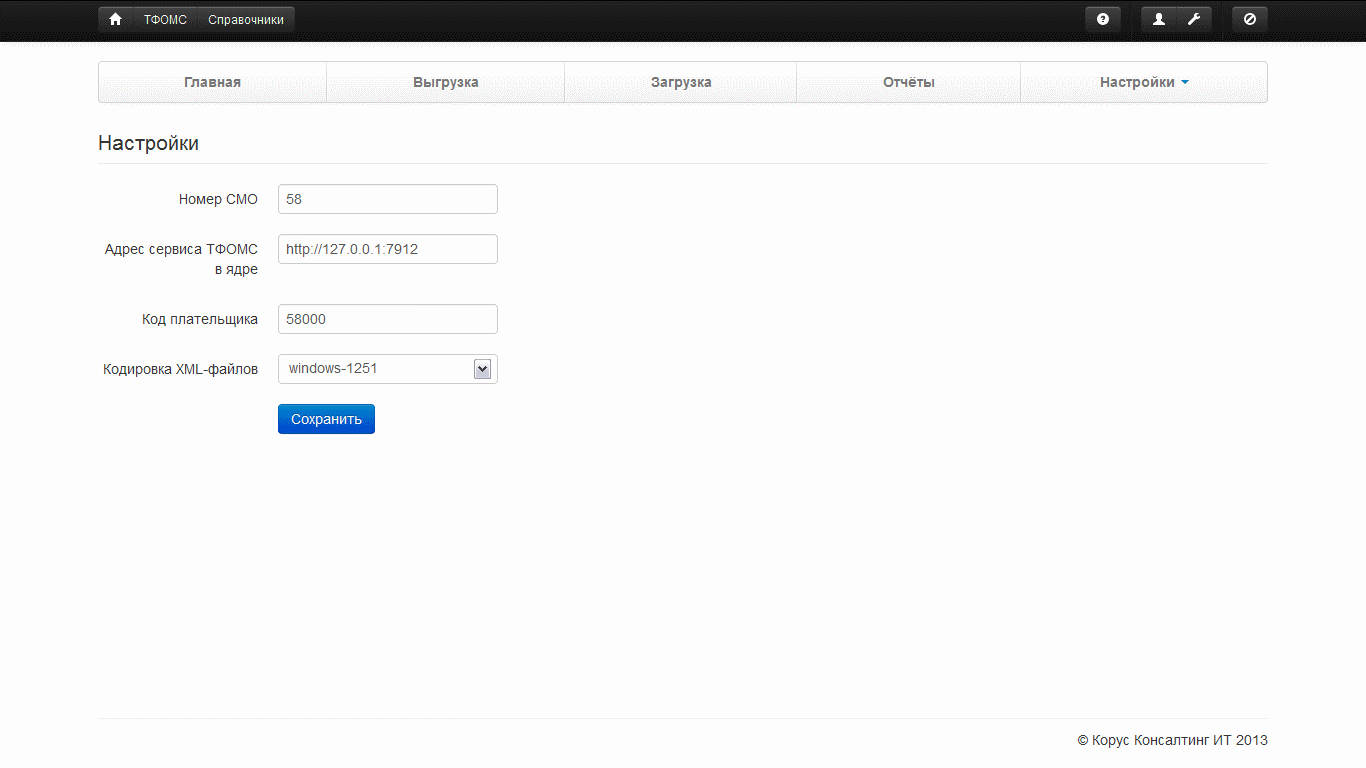
\includegraphics[width = 1\textwidth ,keepaspectratio]{tfoms_conf}
 \caption{Настройки модуля выгрузки в ТФОМС}
 \label{img_tfoms_conf}
\end{figure}

На данной странице содержатся следующие поля:
\begin{itemize}
 \item \dm{Номер СМО} – начальные цифры кодов СМО региона.
 \item \dm{Адрес сервиса ТФОМС в ядре}.
 \item \dm{Код плательщика} – код плательщика для выставления счета.
 \item \dm{Кодировка XML-файлов} выбирается из списка.
\end{itemize}
 
После изменения какой-либо из настроек, необходимо нажать кнопку \btn{Сохранить}.

\subsection{Загрузка ответа от ТФОМС}

Помимо сведений об оплате или отклонении случаев обращении, при передаче результатов проверки выгрузки из ТФОМС могут быть переданы изменения данных полисов пациентов. Например, если переданный полис устарел, то ТФОМС вернет новый действующий полис.

Для обновления данных о полисах пациента используется метод, в который необходимо передать внутренний идентификатор пациента и данные о новом полисе.

При успешном изменении, все предыдущие полисы пациента \textbf{данного типа} будут помечены флагом deleted = 1, а новый полис будет вставлен в таблицу ClientPolicy с комментарием ClientPolicy.note = <<Изменения из ТФОМС>> и признаком deleted = 0.

Если полученные серия или номер полиса превышают 16 знаков, то они будут обрезаны до 16 знаков (ограничение БД).

При изменении данных полиса пациента возможны следующие ситуации:
\begin{itemize}
 \item Переданная связка (серия, номер, тип полиса) является одним из активных полисов пациента – возвращается ошибка о совпадении с текущим полисом.
 \item Отсутствует пациент с переданным идентификатором –возвращается ошибка об отсутствии пациента с указанным идентификатором в БД.
 \item Переданный типа полиса отсутствует в справочнике типов полисов – возвращается ошибка об отсутствии в БД переданного типа полиса.
 \item Во время сохранения полиса возникли ошибки связанные с обращениями к БД – возвращается сообщение о непредвиденной ошибке.
\end{itemize}
